\documentclass[12pt]{article}
 
\usepackage[margin=1in]{geometry}
\usepackage{amsmath,amsthm,amssymb}
\usepackage{listings}
\usepackage{graphicx}
\graphicspath{ {figures/} }
\usepackage{booktabs}
\usepackage{listings}
\usepackage{float}

\newcommand{\N}{\mathbb{N}}
\newcommand{\R}{\mathbb{R}}
\newcommand{\Z}{\mathbb{Z}}
\newcommand{\Q}{\mathbb{Q}}
 
\newenvironment{theorem}[2][Theorem]{\begin{trivlist}
\item[\hskip \labelsep {\bfseries #1}\hskip \labelsep {\bfseries #2.}]}{\end{trivlist}}
\newenvironment{lemma}[2][Lemma]{\begin{trivlist}
\item[\hskip \labelsep {\bfseries #1}\hskip \labelsep {\bfseries #2.}]}{\end{trivlist}}
\newenvironment{exercise}[2][Exercise]{\begin{trivlist}
\item[\hskip \labelsep {\bfseries #1}\hskip \labelsep {\bfseries #2.}]}{\end{trivlist}}
\newenvironment{problem}[2][Problem]{\begin{trivlist}
\item[\hskip \labelsep {\bfseries #1}\hskip \labelsep {\bfseries #2.}]}{\end{trivlist}}
\newenvironment{question}[2][Question]{\begin{trivlist}
\item[\hskip \labelsep {\bfseries #1}\hskip \labelsep {\bfseries #2.}]}{\end{trivlist}}
\newenvironment{corollary}[2][Corollary]{\begin{trivlist}
\item[\hskip \labelsep {\bfseries #1}\hskip \labelsep {\bfseries #2.}]}{\end{trivlist}}
 
\begin{document}
 
\title{Homework HPC}
\author{Ningyu Ma\\ 
ME614 Spring 2017}

\maketitle
\begin{problem}{1}
\text{}\\
$(a)$ From Figure 1, we can see that the truncation error has a 4th order accuracy.\\
The error for using different number of processes cannot be distinguished, they all decay in the order of 4 and slow down when $\Delta x$ is small enough.\\
When $\Delta x$ is small(total number of points $N$ increases), the truncation error seems to be experiencing small random ups and downs due to the accumulation of round off error from each processes. \\
But because float128 floating point precision and small number of processes we are using, the round off error does not play an important role at small  $\Delta x$.\\
\begin{figure}[H]
\centering
  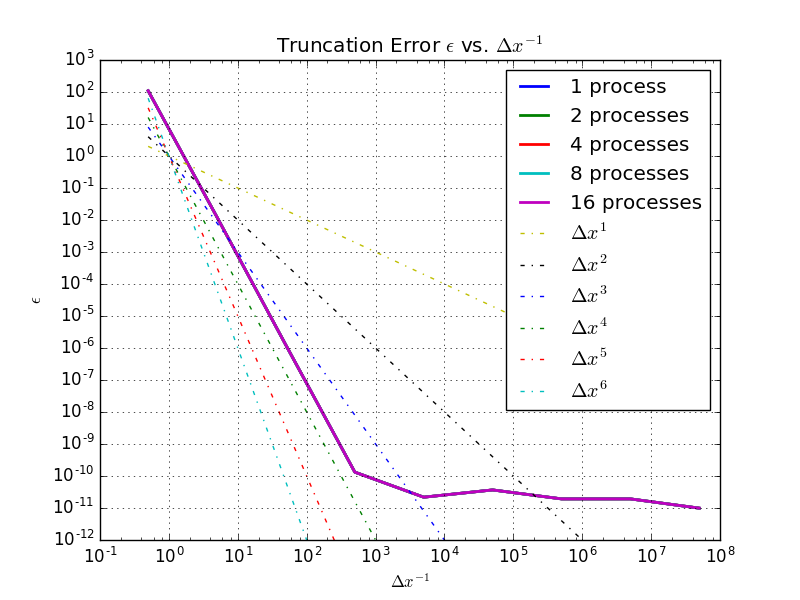
\includegraphics[scale=0.65]{part_a.png}
 \caption{Log-Log Plot for Truncation Error vs. $\Delta x^{-1}$}
\label{label}
\end{figure}
\text{}\\
$(b)$ From Figure 2 and Figure 3, we can see that both the strong and weak scaling efficiencies is experiencing monotonic decrease when the total number of processes($N_{procs}$) increases.\\
\begin{figure}[H]
\centering
  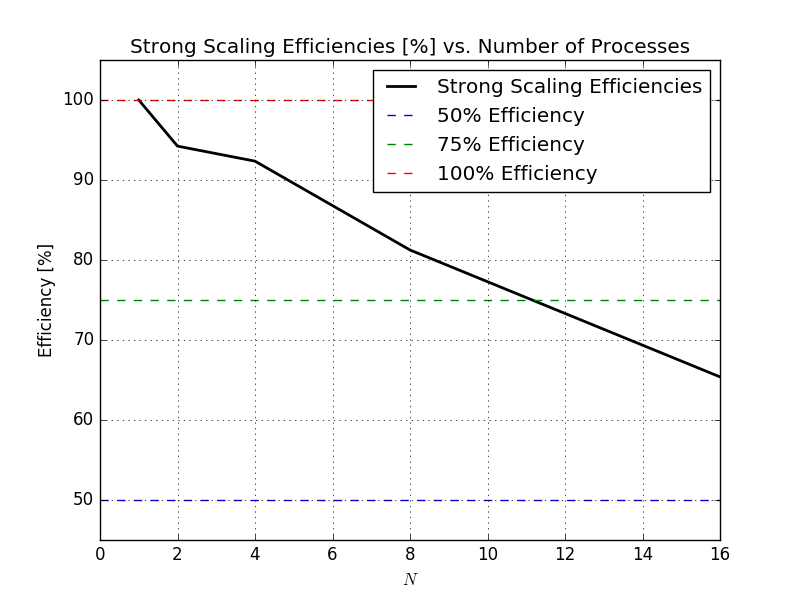
\includegraphics[scale=0.55]{part_b_strong.png}
 \caption{Efficiency Plot for Strong Scaling}
\label{label}
\end{figure}
\begin{figure}[H]
\centering
  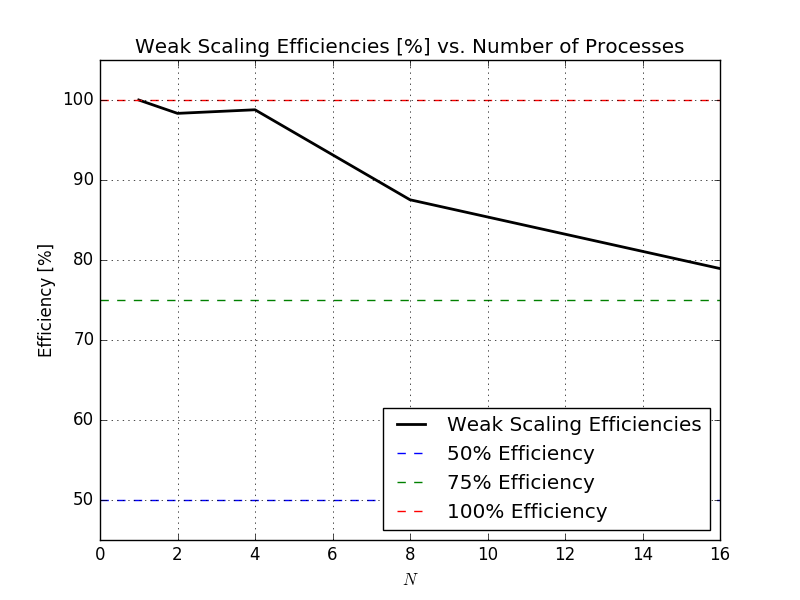
\includegraphics[scale=0.55]{part_b_weak.png}
 \caption{Efficiency Plot for Weak Scaling}
\label{label}
\end{figure}
\text{}\\
$(c)$ From Figure 4 below, we can see that the error varies for each case. At first it decreases w.r.t. increasing number of processes($N_{procs}$).\\
When $N_{procs}$ is large, the error seems to be random because the accumulation of round off error from each processes.\\
\begin{figure}[H]
\centering
  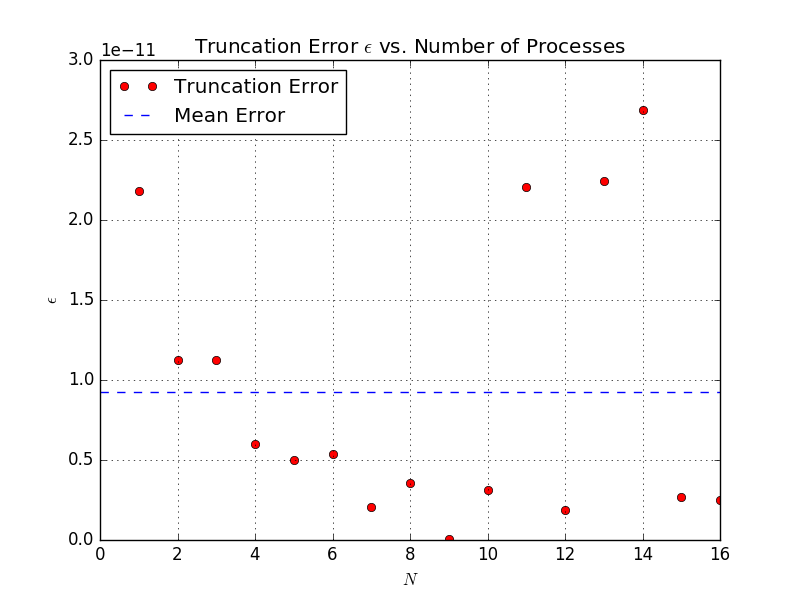
\includegraphics[scale=0.7]{part_c.png}
 \caption{Plot for Truncation Error vs. $N_{procs}$}
\label{label}
\end{figure}
\end{problem}

\end{document}
